\PassOptionsToPackage{unicode=true}{hyperref} % options for packages loaded elsewhere
\PassOptionsToPackage{hyphens}{url}
%
\documentclass[ignorenonframetext,aspectratio=43,]{beamer}

\setbeamercovered{dynamic}
\usepackage[spanish]{babel}
\selectlanguage{spanish}
\uselanguage{Spanish}
\languagepath{Spanish}

\usepackage{pgfpages}
\setbeamertemplate{caption}[numbered]
\setbeamertemplate{caption label separator}{: }
\setbeamercolor{caption name}{fg=normal text.fg}
\beamertemplatenavigationsymbolsempty
% Prevent slide breaks in the middle of a paragraph:
\widowpenalties 1 10000
\raggedbottom
\setbeamertemplate{part page}{
\centering
\begin{beamercolorbox}[sep=16pt,center]{part title}
  \usebeamerfont{part title}\insertpart\par
\end{beamercolorbox}
}
\setbeamertemplate{section page}{
\centering
\begin{beamercolorbox}[sep=12pt,center]{part title}
  \usebeamerfont{section title}\insertsection\par
\end{beamercolorbox}
}
\setbeamertemplate{subsection page}{
\centering
\begin{beamercolorbox}[sep=8pt,center]{part title}
  \usebeamerfont{subsection title}\insertsubsection\par
\end{beamercolorbox}
}
\AtBeginPart{
  \frame{\partpage}
}
\AtBeginSection{
  \ifbibliography
  \else
    \frame{\sectionpage}
  \fi
}
\AtBeginSubsection{
  \frame{\subsectionpage}
}
\usepackage{lmodern}
\usepackage{amssymb,amsmath}
\usepackage{ifxetex,ifluatex}
\usepackage{fixltx2e} % provides \textsubscript
\ifnum 0\ifxetex 1\fi\ifluatex 1\fi=0 % if pdftex
  \usepackage[T1]{fontenc}
  \usepackage[utf8]{inputenc}
  \usepackage{textcomp} % provides euro and other symbols
\else % if luatex or xelatex
  \usepackage{unicode-math}
  \defaultfontfeatures{Ligatures=TeX,Scale=MatchLowercase}
\fi
\usetheme[]{metropolis}
% use upquote if available, for straight quotes in verbatim environments
\IfFileExists{upquote.sty}{\usepackage{upquote}}{}

\IfFileExists{parskip.sty}{%
\usepackage{parskip}
}{% else
\setlength{\parindent}{0pt}
\setlength{\parskip}{6pt plus 2pt minus 1pt}
}
\usepackage{hyperref}
\hypersetup{
            pdftitle={Modelos de computación cuánticos},
            pdfauthor={Pablo Baeyens Fernández},
            pdfborder={0 0 0},
            breaklinks=true}
\urlstyle{same}  % don't use monospace font for urls
\newif\ifbibliography
\setlength{\emergencystretch}{3em}  % prevent overfull lines
\providecommand{\tightlist}{%
  \setlength{\itemsep}{0pt}\setlength{\parskip}{0pt}}
\setcounter{secnumdepth}{0}

% set default figure placement to htbp
\makeatletter
\def\fps@figure{htbp}
\makeatother

\setsansfont[
    Extension      = .otf,
    UprightFont    = *-Light,
    ItalicFont     = *-LightItalic,
    BoldFont       = *-Regular,
    BoldItalicFont = *-RegularItalic
]{FiraSans}
\setmonofont[
    Extension   = .otf,
    UprightFont = *-Regular,
    BoldFont    = *-Medium
]{FiraMono}

\usepackage{appendixnumberbeamer}
\usepackage{svg}
\metroset{titleformat=smallcaps, sectionpage=progressbar, progressbar=frametitle, block=fill}
\definecolor{AzulUGR}{HTML}{007FC0}
\definecolor{RojoUGR}{HTML}{CB2C30}
\setbeamercolor{alerted text}{fg=AzulUGR}
\setbeamercolor{frametitle}{bg=RojoUGR}

\usepackage{tikz}
\usetikzlibrary{arrows}


\newtheorem{teorema}{Teorema}
\newtheorem{corolario}{Corolario}
\newtheorem{lema}{Lema}
\newtheorem{definicion}{Definición}
\newtheorem{problema}{Problema}
\newtheorem{proposicion}{Proposición}
\newtheorem{principio}{Principio}
\newtheorem{ejemplo}{Ejemplo}
\newtheorem{algoritmo}{Algoritmo}

% Bra-ket notation
\newcommand{\bra}[1]{\left\langle#1\right|}
\newcommand{\ket}[1]{\left|#1\right\rangle}
\newcommand{\bk}[2]{\langle #1|#2\rangle}

% Basic commands
\newcommand{\NN}{\mathbb{N}}
\newcommand{\ZZ}{\mathbb{Z}}
\newcommand{\RR}{\mathbb{R}}
\newcommand{\CC}{\mathbb{C}}
\newcommand{\BB}{\mathbb{B}}
\newcommand{\PC}{\mathbb{P}\mathbb{C}}
\newcommand{\norm}[1]{\left\lVert#1\right\rVert}
\newcommand{\set}[2]{\left\{ #1 \;:\; #2 \right\}}

% Complexity
\newcommand{\talph}{\mathcal{T}}
\newcommand{\blank}{\square}
\newcommand{\ew}{\varepsilon}
\newcommand{\TIME}{\operatorname{TIME}}
\newcommand{\SPACE}{\operatorname{SPACE}}
\newcommand{\NTIME}{\operatorname{NTIME}}
\newcommand{\NSPACE}{\operatorname{NSPACE}}
\newcommand{\SIZE}{\operatorname{SIZE}}
\newcommand{\poly}{\operatorname{poly}}
\newcommand{\qeq}{\overset{?}{=}}


\usepackage{listings}

\definecolor{backg}{HTML}{F2F2F2} % Fondo
\definecolor{comments}{HTML}{a8a8a8} % Comentarios
\definecolor{keywords}{HTML}{08388c} % Palabras clave
\definecolor{strings}{HTML}{0489B1}  % Strings

\lstset{
language=haskell,
basicstyle=\small\ttfamily,
breaklines=true,
keywordstyle=\color{keywords},
commentstyle=\color{comments},
stringstyle=\color{strings},
morekeywords={*,Qubit,Circ,QShape,Oracle,QDInt,pure,...},
tabsize=2,
% Acentos, ñ, ¿, ¡ (tex.stackexchange.com/questions/24528)
extendedchars=true,
literate={á}{{\'a}}1 {é}{{\'e}}1 {í}{{\'i}}1 {ó}{{\'o}}1
         {ú}{{\'u}}1 {ñ}{{\~n}}1 {¡}{{\textexclamdown}}1
         {¿}{{?`}}1 {->}{{$\rightarrow$}}1 {\\}{{$\lambda$}}1
         {<-}{{$\leftarrow$}}1
}


\title{Método de ranking en el diseño de un sistema de acceso a la información}
\providecommand{\subtitle}[1]{}
\subtitle{Doble Grado en Ingeniería Informática y Matemáticas}
\author{Johanna Capote Robayna}
\providecommand{\institute}[1]{}
\institute{Trabajo Fin de Grado \\\\\\ \emph{E.T.S. de Ingenierías Informática y de Telecomunicación} \\ \emph{Facultad de Ciencias}}
\date{8 de Julio de 2020}

\usepackage[absolute,overlay]{textpos}
\titlegraphic{
  \begin{textblock*}{3cm}(8.5cm,4.8cm)
    \includesvg[width=3cm]{img/logo-ugr}
  \end{textblock*}
}

\begin{document}
\frame{\titlepage}

\begin{frame}{Índice}
  \begin{columns}[t]
    \begin{column}{.5\textwidth}
      \tableofcontents[sections={1,2}]
    \end{column}
    \begin{column}{.5\textwidth}
      \tableofcontents[sections={3}]
    \end{column}
  \end{columns}
\end{frame}

\section{Introducción}

\begin{frame}{Contextualización}
\begin{itemize}
\item En la década de los 80 Internet empieza a darse a conocer con una primera páginas web.
\pause
\item WebCrawler, Lycos, AltaVista o Yahoo fueron los primeros buscadores.
\pause
\item En 1998 Sergey Brin y Lawrence Page diseñan el algoritmo PageRank.
\end{itemize}
\end{frame}

\section{Matemáticas}
\subsection{Modelo matemático}
\begin{frame}{Modelo matemático}
\begin{center}
Llamamos $P_1, \dots, P_n$ a cada una de las páginas, $n \in \mathbb{N}$. Definimos la importancia $x_i \in [0,1] \subseteq \mathbb{R}$ de la página $P_i$.

Construimos un grafo dirigido donde representamos los enlaces entre las páginas web. Representamos cada página $P_i$ como un nodo y cada enlace de $P_i$ a $P_j$ añadimos una arista de $P_i$ a $P_j$ con una punta de flecha.

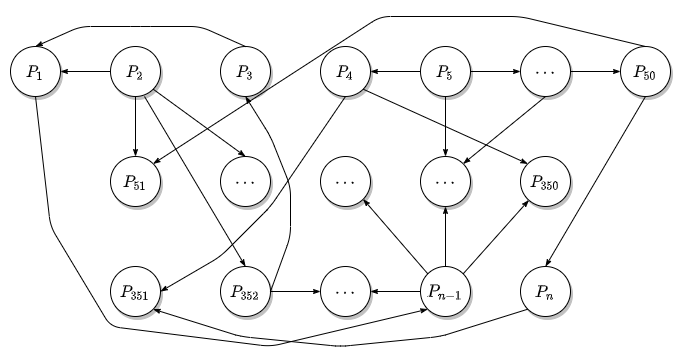
\includegraphics[width=0.8\textwidth]{./img/grafogrande}
\end{center}
\end{frame}

\begin{frame}{Modelo matemático}
\begin{center}
Podemos reflejar esta información en una matriz $M$. Tanto en las filas como en las columnas representamos las $n$ páginas y por cada enlace entre una página $j$ a otra página $i$, escribimos un 1 en la entrada de la matriz $m_{ij}$ y en el caso de que no haya enlace escribimos un 0.

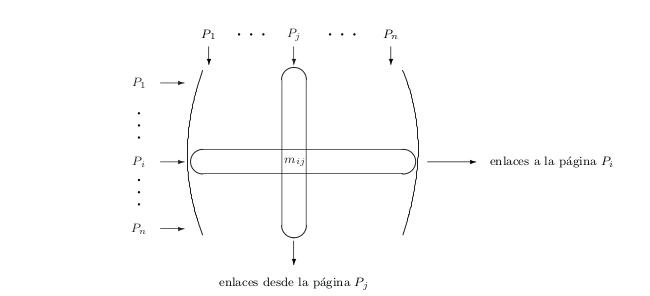
\includegraphics[width=1.0\textwidth]{./img/matriz}
\end{center}
\end{frame}

\begin{frame}{Modelo matemático}
\begin{itemize}
\item Primera aproximación: la importancia de una página web es proporcional al número de enlaces entrantes.
\item Problema: el número de enlaces no representa del todo la importancia. No es lo mismo que la página este citada por una página cualquiera que por una página ``importante'' como \textbf{www.facebook.com} o \textbf{www.apple.com}.
\item Solución: definimos que la importancia de una página web $x_j$ es proporcional a la suma de las importancias de las páginas que enlazan con $P_j$.

\end{itemize}

\end{frame}

\begin{frame}{Modelo matemático}
\begin{center}
Supongamos, por ejemplo, que la página $P_1$ es citada desde las páginas $P_{200}$ y $P_n$, que $P_2$ se cita desde $P_1$, $P_{200}$ y $P_{n-1}$, mientras que en la última página $P_n$ hay enlaces desde $P_1$, $P_2$, $P_{50}$, $P_{200}$ y $P_{n-1}$. En nuestra asignación anterior, $x_1, \dots, x_n$ deberían cumplir entonces que:
$$ x_1 = K(x_{200} + x_n) $$
$$ x_2 = K(x_1 + x_{200} + x_{n-1})$$
$$ \vdots $$
$$ x_n = K(x_1 + x_2 + x_{50} + x_{200} + x_{n-1})$$
donde $K$ es una constante de proporcionalidad.
\end{center}

\end{frame}

\begin{frame}{Modelo matemático}
\begin{center}
Escribimos el sistema de ecuaciones anterior en términos matriciales.
$$ $$
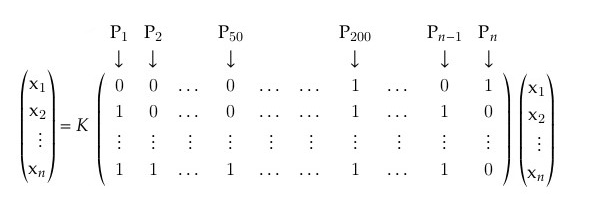
\includegraphics[width=1.0\textwidth]{./img/matrizejemplo}
Si llamamos $\vec{x}$ al vector de importancias $(x_1,\dots, x_n)$, $\lambda = \frac{1}{K}$ y $M$ a la matriz asociada al grafo. Nos encontramos con un problema de valores propios y vectores propios:
$$M \vec{x} = \lambda \vec{x} $$
\end{center}
\end{frame}

\subsection{Teorema de Perron-Frobenius}

\begin{frame}{Teorema de Perron-Frobenius}
\begin{definicion}[Valor propio dominante]
Sea $A \in M_n(\mathbb{C})$, se dice que tiene valor propio dominante si el espectro
$$\sigma (A) = \{ \lambda_1, \lambda_2 \dots \lambda_n \} \   (r \leq n)$$
cumple:
\begin{itemize}
\item $\lambda_1 > 0$.
\item $m(\lambda_1) = 1$.
\item $|\lambda_i| < \lambda_1$ para $i = 2, \dots , r$.
\end{itemize}
\end{definicion}
Al valor propio dominante lo notaremos como $\lambda_p$.
\end{frame}

\begin{frame}{Teorema de Perron-Frobenius}
\begin{proposicion} Sea $A \in M_n(\mathbb{C})$ una matriz con valor propio dominante $\lambda_p$. Entonces el límite $\lim_{k \to \infty} \frac{1}{\lambda_p^k}A^k = Q$ donde $Q \in M_n(\mathbb{C})$ que cumple:
$$ImQ = Ker ( A - \lambda_p I) \ , Q^2 = Q \ , QA = AQ $$
Se dice que $Q$ es una $\textrm{proyección espectral de A}$.
\end{proposicion}


\end{frame}

\subsubsection{Matrices positivas}

\begin{frame}{Matrices positivas}
\begin{teorema}[Perron, 1907]
\label{perron}
Sea $A \in M_n(\mathbb{C})$, $A > 0$ con $\lambda_p = \rho(A)$. Entonces:
\begin{enumerate}
\item $\lambda_p >0$.
\item $\lambda_p \in \sigma(A)$ ($\lambda_p$ es llamado raíz de Perron).
\item $m(\lambda_p) = 1$.
\item Existe un vector propio $\vec{v} >0$ tal que $A\vec{v} = \lambda_p \vec{v}$.
\item El $\textrm{vector de Perron}$ es el único definido como
$$A\vec{p} = \lambda_p \vec{p} \ , \vec{p} > 0 \ , \textrm{y} \ \|\vec{p}\|_1 = 1 $$
y, excepto los múltiplos positivos de $\vec{p}$, no hay otros vectores propios no negativos para $A$, independientemente del valor propio.
\item $\lambda_p$ es el único valor propio en el circulo espectral de $A$.
\end{enumerate}
\end{teorema}
\end{frame}

\subsubsection{Matrices no negativas}

\begin{frame}{Matrices no negativas}

\begin{definicion}[Matriz reducible]
Se dice que una matriz $A \in M_n(\mathbb{R})$ no negativa ($A \geq 0$) es reducible si existe una permutación simétrica (de filas y columnas) que transforma $A$ en una matriz del tipo:
$$\left(
      \begin{array}{{c|c}}
            A_{11}    &    A_{12}  \\\hline
            0         &    A_{22}     \\
      \end{array}   \right)$$
donde $A_{11}$ y $A_{22}$ son matrices cuadradas. Una matriz se dice irreducible cuando no es reducible.
\end{definicion}
\end{frame}

\begin{frame}{Matrices no negativas}
\begin{proposicion}
\label{irreducible}
\label{positiva}
Sea $A \in M_n(\mathbb{R})$ una matriz no negativa ($A \leq 0$). Son equivalentes:
\begin{enumerate}
\item A es irreducible.
\item La matriz $(I + A)^{n - 1}$ es positiva.
\item Si $A$ es la matriz de adyacencia de un grafo, entonces el grafo está fuertemente conectado.
\end{enumerate}
\end{proposicion}

\begin{definicion}[Grafo fuertemente conectado]
Un grafo dirigido $G$ se dice fuertemente conectado si para cada par de nodos distintos $P_i$, $P_j$ en $G$ hay un camino de longitud finita que comienza en $P_i$ y termina en $P_j$.
\end{definicion}
\end{frame}

\subsubsection{Enunciado del teorema}

\begin{frame}{Enunciado del teorema}
\begin{teorema}[Frobenius, 1908-1912]
Sea $A $ una matriz cuadrada ($A \in M_n(\mathbb{C})$) no negativa ($A \geq 0$). Si $A$ es irreducible, entonces para $r = \rho(A)$ se cumple que:
\begin{enumerate}
\item $r >0$ , $r \in \sigma(A)$ y
\item $m(r) = 1$.
\item Existe un vector propio $\vec{x} > 0$ asociado a $r$.
\item El único vector definido por:
$$A \vec{p} = r \vec{p}  \ , \ \vec{p}> 0 \ , \textrm{y} \ \|\vec{p}\|_1 = 1 $$
es el vector de Perron. No hay ningún vector propio no negativo para $A$ excepto los múltiplos positivos de $\vec{p}$, independientemente del valor propio.
\end{enumerate}
\end{teorema}
\end{frame}

\subsubsection{Método de las potencias}

\begin{frame}{Método de las potencias}
El método de las potencias comienza con un vector inicial $\vec{x}^{(0)} \in \mathbb{R}^n  \ , \vec{x}^{(0)} \geq 0$, para calcular los siguiente $\vec{x}^{(k)}$ se utiliza la siguiente fórmula recurrente:
$$\vec{x}^{(k+1)} = A \vec{x}^{(k)} \textrm{ con } k \in \mathbb{N}$$ esta fórmula la podemos desarrollar obteniendo  $$\vec{x}^{(k)} = A^k \vec{x}^{(0)}$$
Se puede demostrar que
$$\lim_{k \to \infty} \frac{1}{\|\vec{x}^{(k)}\|_1} \vec{x}^{(k)} = \vec{p} $$
Siendo $\vec{p}$ el vector de Perron de $A$.
\end{frame}


\section{Informática}

\subsection{Modificaciones previas}
\begin{frame}{Modificaciones previas}

Supongamos que el usuario se encuentra navegando por la red, por ejemplo, en la primera página $P_1$ y cuando se aburre decide saltar a una de las páginas con las que enlaza $P_1$ . Supongamos que hay $N_1$ páginas que enlazan desde $P_1$ , es lógico pensar que todas tienen una probabilidad de ser elegidas del $\frac{1}{N_1}$ es decir que siguen una distribución de probabilidad uniforme (discreta) en $[ 1, N_1 ]$.
\begin{center}
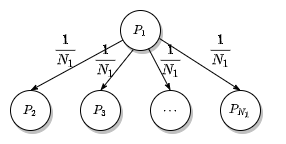
\includegraphics[width=0.5\textwidth]{./img/grafoprobini}

\end{center}
\end{frame}

\begin{frame}{Modificaciones previas}
\begin{center}
Volvemos a considerar las mismas paginas web $P_1, P_2, \dots, P_n$ y $M$ la matriz de adyacencia del grafo, cuyas entradas $m_{ij}$ son 0 y 1. Llamamos $N_j$ al número de enlaces de la página $P_j$ , es decir al número de entradas de la columna $j$. Construimos una nueva matriz $M'$ a partir de la $M$ original sustituyendo cada $m_{ij}$ por:
$$m'_{ij} = \frac{m_{ij}}{N_j} $$

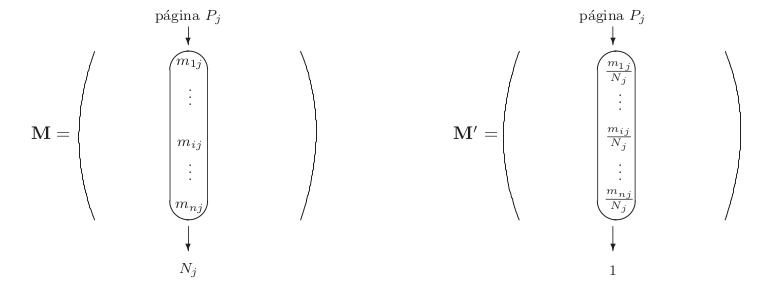
\includegraphics[width=1.0\textwidth]{./img/markov}
\end{center}
\end{frame}

\begin{frame}{Modificaciones previas}
Con este modelo podemos conocer con que probabilidad estará el usuario en cada una de las páginas tras cada instante de tiempo, entendiendo instante de tiempo como transiciones o saltos.
Si multiplicamos $M'$ por el vector inicial, obtenemos:
$$\begin{pmatrix}
\cdots & \cdots & m'_{1k} & \cdots \\
\vdots & \ddots & \vdots & \vdots \\
\cdots & \cdtos & m'_{kk} & \cdots \\
\vdots & \vdots & \vdots & \ddots \\
\cdots & \cdots & m'_{nk} & \cdots \end{pmatrix} \begin{pmatrix}
0 \\
\vdots \\
1 \\
\vdots \\
0 \end{pmatrix} = \begin{pmatrix}
m'_{1k}\\
\vdots \\
m'_{kk} \\
\vdots \\
m'_{nk} \end{pmatrix}$$
Este vector resultante, cuyas entradas son o 0 o $\frac{1}{N_k}$, describe con que probabilidad estará el usuario en cada una de las páginas tras una unidad de tiempo.
\end{frame}
\begin{frame}
\begin{itemize}
\item \textbf{Problema}: Sin embargo, podría ocurrir que alguna de las páginas no citaran a ninguna otra, es decir, que ese nodo del grafo no tuviera enlaces salientes. Esto se traduce en que en nuestra matriz $M'$ aparece una columna de ceros, por lo que esta matriz dejaría de ser primitiva y además el grafo del que partimos no estaría fuertemente conectado.
\item \textbf{Solución}:
$$M'' = cM' + (1-c)\begin{pmatrix}
p_1 \\
\vdots \\
p_n \end{pmatrix} (1, \dots, 1)$$
Donde $p_1 , \dots , p_n$ es una distribución de probabilidad y c es un parámetro entre 0 y 1. La distribución de probabilidad a que elegimos es una distribución uniforme que asigne una probabilidad de $p_i = 1/n$.
\end{itemize}
\end{frame}

\subsubsection{Modelo Booleano}
\begin{frame}{Modelo Booleano}
Definimos:
\begin{itemize}
\item El conjunto de todos los términos de la colección de documentos como $V = \{t_1, t_2, \dots, t_M\}$
\item El conjunto de todos los documentos de la colección como $D = \{d_1,d_2, \dots, d_N\}$.
\item Para cada término $t_i$ se define $T_i$ como el conjunto formado por todos los documentos que contienen el término $t_i$.
\end{itemize}
\end{frame}

\begin{frame}{Modelo Booleano}
Si por ejemplo tuvieramos los siguientes cuatro documentos:
\begin{itemize}
\item $d_1 = $ \{gato, gato, gato, tortuga, pez\}
\item $d_2 = $ \{perro, caballo\}
\item $d_3 = $ \{gato, perro, águila\}
\item $d_4 = $ \{pez, tortuga, tortuga\}
\end{itemize}
Entonces la consulta obtendría el siguiente resultado:
\begin{itemize}
\item $\textrm{perro AND gato } = T_1 \cap T_2 = \{d_2, d_3\} \cap \{d_1, d_3\} = \{d_3\}$
\item $\textrm{perro OR gato } = T_1 \cup T_2 = \{d_2, d_3\} \cup \{d_1, d_3\} = \{d_1, d_2, d_3\}$
\item $\textrm{perro OR NOT gato } = T_1 \cup (D - T_2) = \{d_2, d_3\} \cup \{d_2, d_4\} = \{d_2, d_3, d_4\}$
\end{itemize}
\end{frame}

\begin{frame}{Modelo Booleano}
\begin{itemize}
\item \textbf{Ventajas}
\begin{itemize}
\item Sencillez.
\item Flexibilidad.
\end{itemize}
\item \textbf{Inconvenientes}
\begin{itemize}
\item No se tiene en cuenta la frecuencia del término en el documento.
\item No se tiene en cuenta la relevancia del término.
\end{itemize}
\end{itemize}
\end{frame}

\subsubsection{Modelo vectorial}
\begin{frame}{Modelo vectorial}
Definimos:
\begin{itemize}
\item El conjunto de todos los términos de la colección de documentos como $V = \{t_1, t_2, \dots, t_M\}$
\item El conjunto de todos los documentos de la colección como $D = \{d_1,d_2, \dots, d_N\}$.
\item Un documento $\vec{d}_j$ como un vector, de tamaño el número de términos, $\vec{d}_j = (w_{1,j}, w_{2,j}, \dots , w_{M,j})$ donde $w_{i,j}$ indice el peso del término $i$ en el documento $j$.
\end{itemize}
\begin{center}
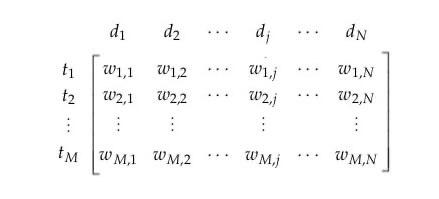
\includegraphics[scale=0.4]{./img/matrizpesos}
\end{center}
\end{frame}

\begin{frame}{Modelo vectorial}
Este modelo se basa en dos conceptos fundamentales:
\begin{itemize}
\item Esquema de pesos.
\item Similitud entre dos vectores de términos (por ejemplo, entre un documento y una consulta).
\end{itemize}
$$sim(\vec{q},\vec{d}) = cos(\alpha) = \frac{\sum_{i = 1}^M w_{i,q} \cdot w_{i,d}}{\sqrt{\sum_{i = 1}^M w_{i,d}^2} \cdot \sqrt{\sum_{i = 1}^M w_{i,q}^2}} = \frac{\vec{q}}{|\vec{q}|} \cdot \frac{\vec{d}}{|\vec{d}|} $$
$$ \textrm{ donde } |\vec{v}| = \sqrt{\sum_{i = 1}^M v_i^2}$$
\end{frame}

\begin{frame}{Modelo vectorial}
A la hora de calcular el peso de un término en cada documento debemos tener en cuenta dos conceptos:
\begin{itemize}
\item La frecuencia del término en el documento.
\item La especificidad del término en el documento.
\end{itemize}

\end{frame}

\begin{frame}{Modelo vectorial}
Por lo tanto, calcularemos el peso de un término de la siguiente forma:
$$w_{i,j} = tf_{i,j} \cdot idf_i = tf_{i,j} \cdot \log \left(\frac{N}{n_i} \right) $$


Tras calcular estos pesos se normaliza cada vector $\vec{d}_j$:
$$\vec{d}_j = \frac{\vec{d}_j}{|\vec{d}_j|} $$
\end{frame}

\begin{frame}{Modelo vectorial}
Procedimiento:
\begin{itemize}
\item \textbf{Antes de introducir la consulta:}
\begin{itemize}
\item Se calculan la matriz de pesos.
\end{itemize}
\item \textbf{Introducida la consulta:}
\begin{itemize}
\item Se calculan los pesos de la consulta $\vec{q}$.
\item Se calcula la similitud de la consulta $\vec{q}$ con cada documento de la colección. Se obtiene un vector de relevancias donde queda reflejada la similitud de cada documentos a la consulta.
\item Se multiplica el vector de relevancias por el vector del PageRank.
\end{itemize}
\end{itemize}

\end{frame}

\subsubsection{Técnicas de modificación de la consulta}
\begin{frame}{Técnicas de modificación de la consulta}
\underline{\textbf{Realimentación de consultas}}


El objetivo de esta técnica consiste en conseguir una consulta expandida $\vec{q}'$ a partir de una consulta $\vec{q}$, para ello se utiliza la fórmula de Rocchio:
$$\vec{q}' = \alpha \vec{q} + \frac{\beta}{D_r} \sum_{\vec{d}_j \in D_r} \vec{d}_j - \frac{\gamma}{D_{nr}} \sum_{\vec{d}_j \in D_{nr}} \vec{d}_j $$

 Usualmente se le da valores $\alpha = 1$, $\beta = 0.75$ y $\gamma = 0$, ya que no buscamos ampliar la consulta con documentos no relevantes.
\end{frame}

\subsection{Ejemplo}
\begin{frame}{Ejemplo}
\underline{Quinto clasificado}
\begin{itemize}
\item Título: Neuroimaging Endpoints in Amyotrophic Lateral Sclerosis.
\item ORCID autor: 0000-0003-0267-3180
\item Abstract: Amyotrophic lateral \colorbox{yellow}{sclerosis} ...
\end{itemize}

\underline{Decimo clasificado}
\begin{itemize}
\item Título: \colorbox{yellow}{Pathology} and MRI: exploring cognitive impairment in MS.
\item ORCIRD autor: 0000-0002-6378-0070
\item Abstract: Cognitive impairment is a frequent symptom in people with multiple \colorbox{yellow}{sclerosis}, affecting up to 70\% of \colorbox{yellow}{patients}...
\end{itemize}
\end{frame}

\subsection{Conclusiones y trabajos futuros}
\begin{frame}{Conclusiones y trabajos futuros}
\begin{itemize}
\item \textbf{Conclusiones:}
\begin{itemize}
\item Se resuelve el problema de ordenar información según el interés del usuario.
\item Se consiguen personalizar las búsquedas.
\end{itemize}
\item \textbf{Trabajos futuros:}
\begin{itemize}
\item Crear perfiles de usuario.
\item Modificar el software para que sea más escalable.
\item Paralelizar el software para conseguir trabajar con conjunto más grandes.
\end{itemize}
\end{itemize}
\end{frame}
\begin{frame}[standout]

Gracias por su atención
\end{frame}

\end{document}
